%% IMPORTANT: Once working, run latex 3 times to get listoffigures to work

%% Be sure to check spelling!

%% Put your name and the proper due date in place

%% Copy the lstinputlisting and figure code as many times as you need
%% Be sure to put in your own file names if appropriate

%% Note that the \epsfig and \lstinputlisting commands 
%% are currently commented out with %%% - until the
%% files exist, processing this code without them will result in an error
%% so leave the comments until you have created the files!

\documentclass{article}
\usepackage{amsmath}    % loads AMS-Math package
\usepackage{epsfig}     % allows PostScript files
\usepackage{listings}   % allows lstlisting environment
\usepackage{moreverb}   % allows listinginput environment
\usepackage[letterpaper, margin=0.75in]{geometry}  % set paper size/margins
\usepackage{EGR103F19}  % colorful file imports

\begin{document}
\begin{center}
\rule{6.5in}{0.5mm}\\~\\
\textbf{\large EGR 103L -- Fall 2019}\\~\\
\textbf{\huge Lab 5: Structured Programming II}\\~\\
***NAME (NetID)***\\
***Lab Section N, DAY TIMES***\\
***DATE DUE***\\~\\
{\small I understand and have adhered to all the tenets of the Duke
  Community Standard in completing every part of this assignment.  I
  understand that a violation of any part of the Standard on any part
  of this assignment can result in failure of this assignment, failure
  of this course, and/or suspension from Duke University.} 
\rule{6.5in}{0.5mm}\\
\end{center}
\tableofcontents
%\listoffigures
\pagebreak

\section{P\&E 4.46}
%%% Uncomment this once you have the file
%%% \lstinputlisting[basicstyle=\ttfamily]{Coded.txt}

\section{P\&E 4.49}
%%% Uncomment this once you have the file
%%% \lstinputlisting[basicstyle=\ttfamily]{dcs_scramble.txt}

\section{Chapra 4.25}
%%% Write a few sentences about anything interesting you see with 
%%% the graphs.

\section{Finding Roots}
%%%  Write a few sentences about anything interesting you see with 
%%% the graphs as well as what you perceive to be the advantages 
%%% and disadvantages of presenting the information as plots in 
%%% Figure 1 versus images in Figure 2.

\pagebreak
\appendix
\section{Codes}
% Put the name of your file in the subsection name 
% and the listinginput input
% Be sure to include the community standard in codes!
% Add \pagebreaks if they make sense

%%% Uncomment as needed

\lstset{style=python103, language=python} 

\subsection{swap\_letters.py}
%%%\lstinputlisting{swap_letters.py}
\clearpage

\subsection{scrambler.py}
%%%\lstinputlisting{scrambler.py}
\clearpage

\subsection{cos\_series.py}
%%%\lstinputlisting{cos_series.py}
\clearpage

\subsection{poly\_root.py}
%%%\lstinputlisting{poly_root.py}
\clearpage 

% start Figures on new page

\section{Figures}
\begin{figure}[ht!]
\begin{center}
\begin{tabular}{cc}
%%%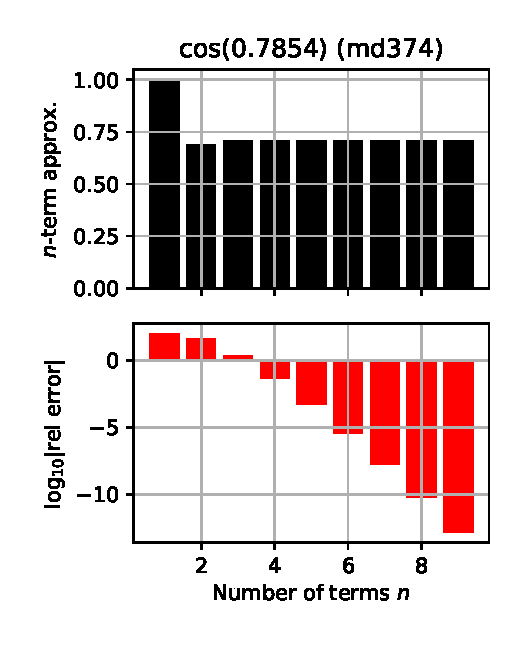
\epsfig{file=CosPlot0.eps} &
%%%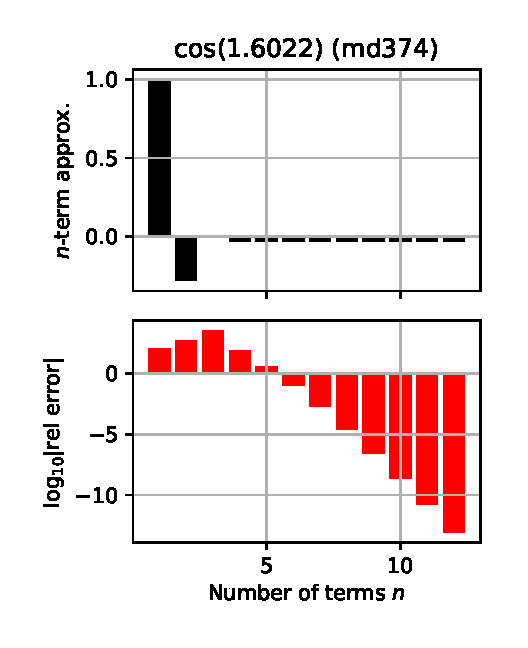
\epsfig{file=CosPlot1.eps} \\
%%%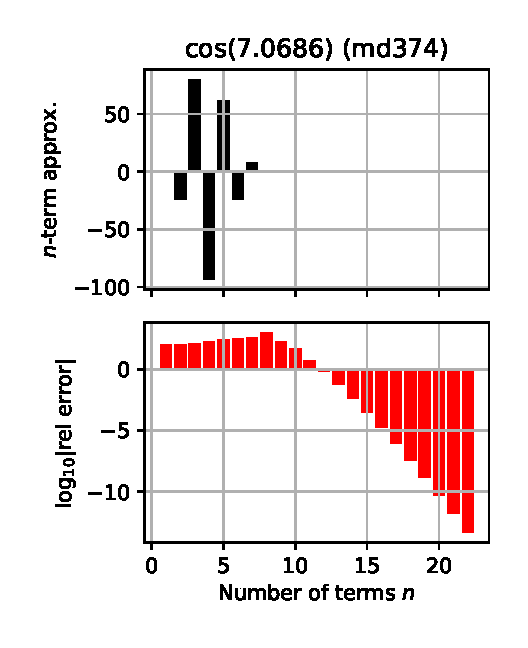
\epsfig{file=CosPlot2.eps} &
%%%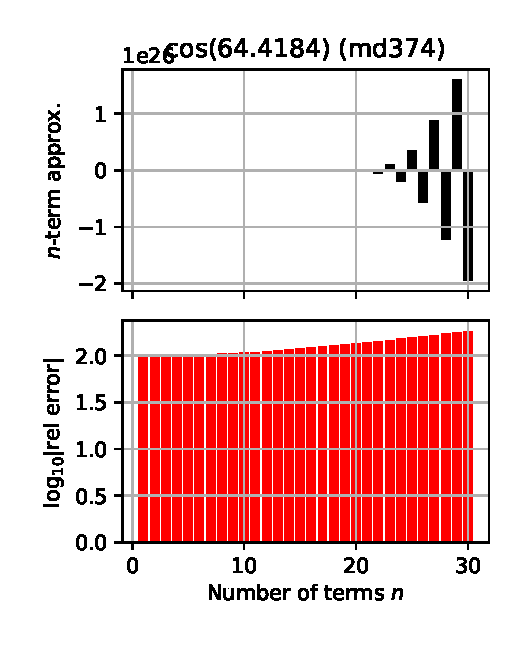
\epsfig{file=CosPlot3.eps} 
\end{tabular}
\caption{Figures for Cosine Approxmiation}
\end{center}
\end{figure}
\clearpage
\begin{figure}[ht!]
\begin{center}
%%%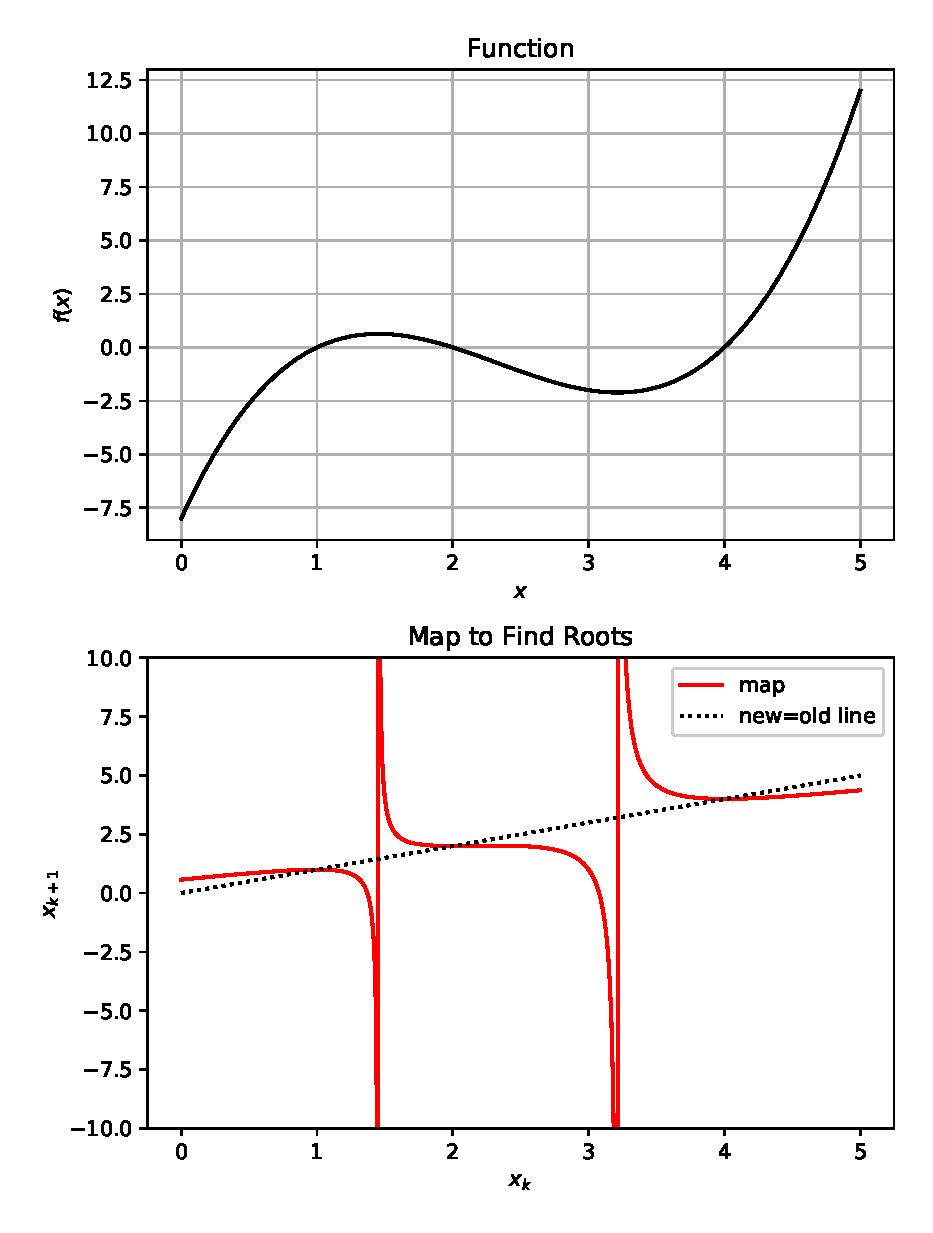
\epsfig{file=RootPlot0.eps} 
\caption{Function and Derivative}
\end{center}
\end{figure}
\begin{figure}[ht!]
\begin{center}
%%%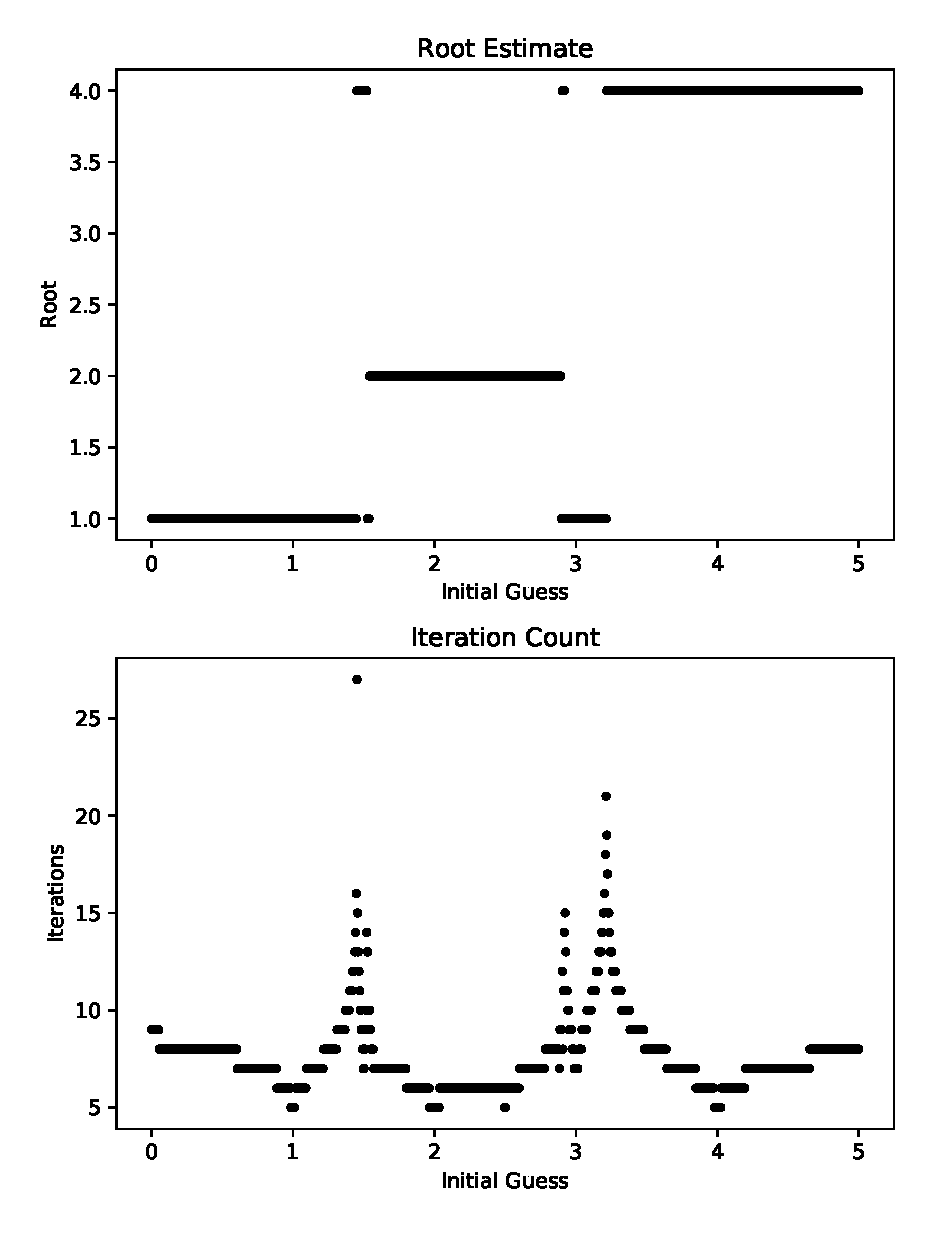
\epsfig{file=RootPlot1.eps} 
\caption{Root Estimates and Iteration Count}
\end{center}
\end{figure}
\begin{figure}[ht!]
\begin{center}
%%%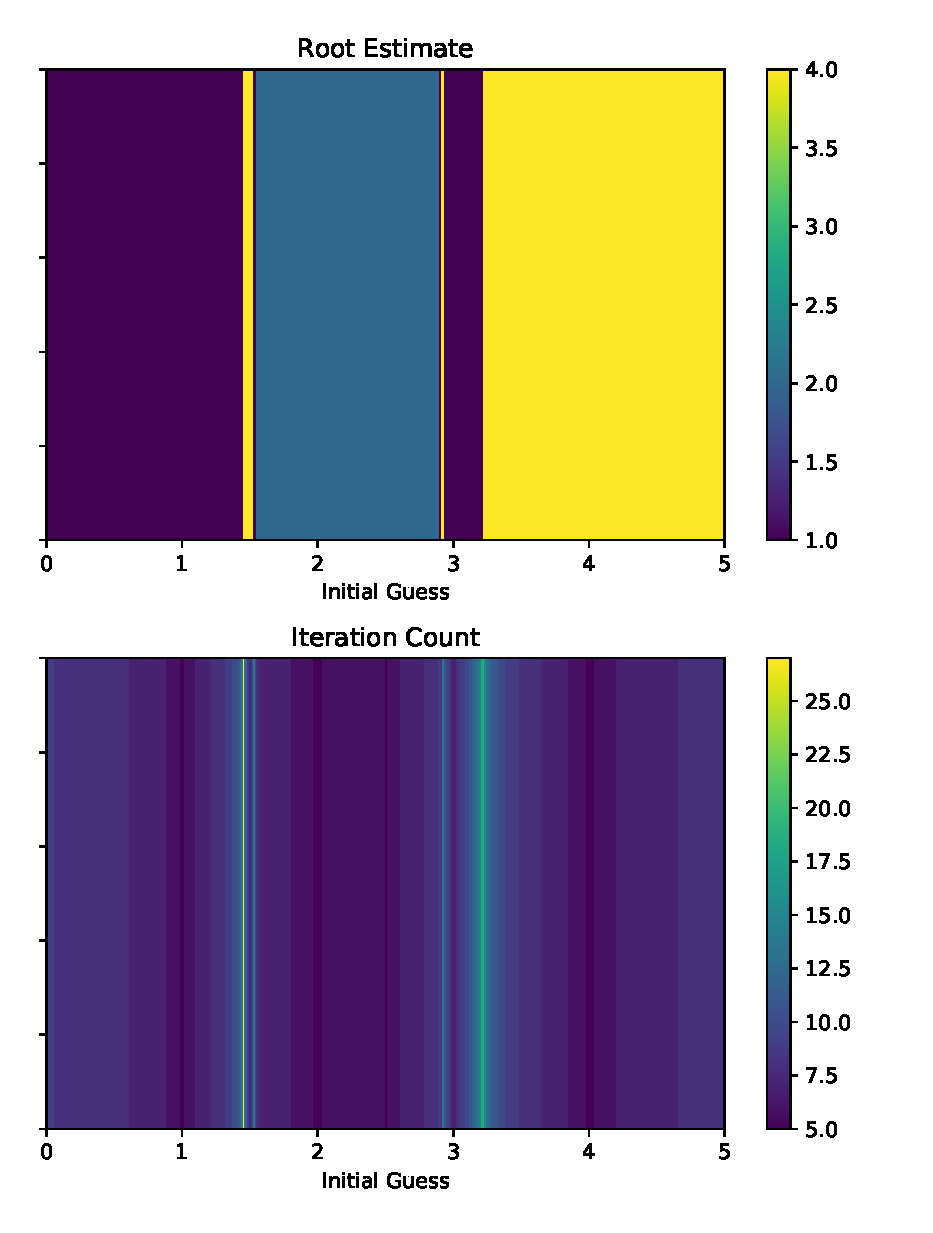
\epsfig{file=RootPlot2.eps} 
\caption{Root Estimates and Iteration Count - As Image}
\end{center}
\end{figure}

\end{document}

